\chapter{Evaluation and Results} \label{chap:evaluation}
\ldots
Unfortunately, there are no publicly available benchmarks for 360\degree image synthesis or image-based rendering for comparison with other methods. Instead, this chapter presents a basic evaluation of the algorithm presented in Chapter~\ref{chap:implementation} that assesses the effects of different parameters on the accuracy of the resulting image compared to the ground truth by using mathematically calculable error metrics. Furthermore, it compares the results of regular blending, flow-based blending, and a naive baseline algorithm to analyze whether, and in which cases an improvement could be achieved.

First, possible parameters are presented \ldots \todo{structure of the chapter}

%First the evaluation methodology is presented, outlining how the effects of a parameter are measured and evaluated. Then, the limits of the algorithm are explored using virtual scenes. With the information gleaned from this limit evaluation, the parameters are chosen for a proof-of-concept evaluation using real scenes. The results and limitations are then discussed\ldots

%- what is a scenario what is a scene
%- not performance
%- konkreter
%- wie gut koennen szenen synthetisiert werden
%- scope: basic evaluation of mathematically measurable values (no human perception)
%- these datasets could be used in the future to compare different algorithms

\section{Parameters}
Before defining the parameters to test in the limitation and proof-of-concept evaluations, this section gives an overview of possible parameters in the context of the 2DoF algorithm presented in Chapter~\ref{chap:implementation}.
The 2DoF algorithm already makes a few assumptions, for example the constraint to the viewpoint plane, the fact that the scene is static, and more (stated in Section \ref{sec:approach} on page \pageref{sec:approach}). These assumptions are upheld in the evaluation, as they are prerequisite to the function of the algorithm.

The remaining parameters (that are not constrained by the assumptions) can be divided into two categories: internal parameters (i.e. based within the algorithm), such as the blending type and the selection of input viewpoints, and external parameters (i.e. based on the properties of the captured scene), such as the viewpoint density, or the geometry of the scene. The internal parameters can be modified after the scene has been captured, the external ones cannot.

The most prominent internal parameters based on the implementation from Chapter~\ref{chap:implementation} are:
\begin{itemize}
  \item the location of synthesized points within the scene (near walls, objects, etc)
  \item the blending type, i.e. flow-based blending or deviation-angle-based knn blending (``regular blending'')
  \item the selection of input viewpoints from the available captured viewpoints
  \item the optical flow algorithm used for flow-based blending
\end{itemize}

There are more internal parameters that could theoretically be modified, such as the knn blending function (the inverse sigmoid function on page~\pageref{eq:sigmoid}), or the method of approximation for 2DoF in flow-based blending (page~\pageref{subsec:2dof_flow-based}), but these will be assumed immutable for this evaluation, as the variation of these parameters would require developing new functions, which would be outside the scope of this thesis.

As for the possible external parameters, the number of different possible scenes is infinite, but the assumed key parameters are:
\begin{itemize}
  \item type of scene (outdoor, indoor, etc) \ar size and shape of scene
  \item objects within the scene
  \item density of captured viewpoints
  \item distribution of captured viewpoints
\end{itemize}

External parameters such as the camera settings (e.g. aperture, shutter speed, white balance) and the lighting throughout the scene are not considered; it is assumed that all the captures have the same camera settings and the white balance is comparable throughout the scene. Furthermore, the evaluation is restricted to indoor scenes of average size (approximately between $4m^2$ and $36m^2$). This reduces the parameter space significantly, since the scale of indoor scenes contains much less variance, since rooms tend to be enclosed by walls.

The evaluation presented in this thesis aims to examine the effects of a few select internal and external parameters, instead of exhaustively examining all of them. In order to do this, a \emph{scenario} is designed for each selected parameter that attempts to demonstrate the effect of this parameter on the accuracy of the result. Limiting the evaluation to specific scenarios reduces the testing space but might also lead to missing some interactions between parameters. This is acceptable, since the evaluation does not aim to be comprehensive. 

%The scenario definition is the first step of the evaluation process which is presented in the next section.
%The parameters to be evaluated, along with their corresponding scenarios depend on the type of evaluation

\section{Evaluation Methodology}
The evaluation is divided into two distinct phases: an evaluation of limits using virtual scenes, and a proof-of-concept evaluation using real scenes. Both evaluations follow the methodology depicted in Figure~\ref{fig:eval-methodology}, and consist of four steps: \emph{scenario definition}, where a scenario is designed to exemplify the parameter to test, \emph{synthesis}, where the synthesized images are calculated using the 2DoF synthesis presented in Chapter~\ref{chap:implementation}, \emph{error calculation}, where the accuracy of the synthesized images is measured, and \emph{result analysis}, where the the cause and effect of the parameters is examined. The details of these steps are described in the following sections.

\begin{figure}
		\centering
		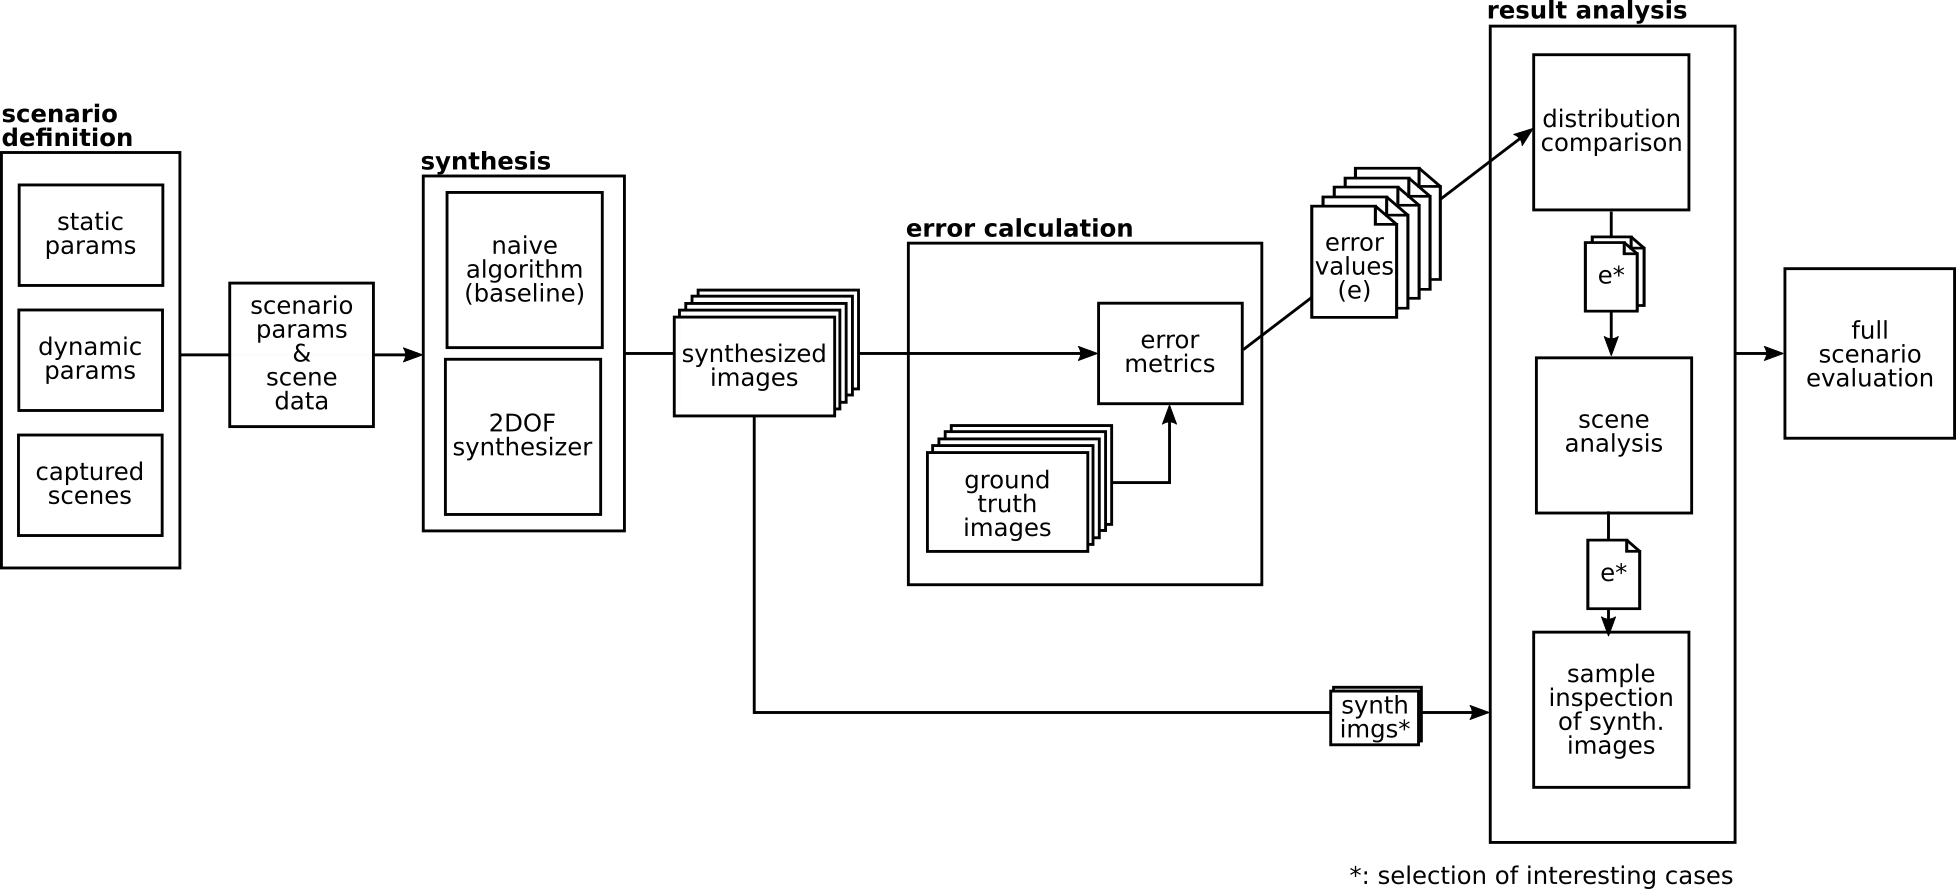
\includegraphics[width=\textwidth]{04/eval_methodology.png}
		\caption{Methodology for the evaluation of a scenario}
		\label{fig:eval-methodology}
\end{figure}

\subsubsection{Scenario Definition}
Since only In order to do this, a \emph{scenario} is designed for each selected parameter that attempts to demonstrate the effect of this parameter on the accuracy of the result.

First, a scenario must be defined that illustrates the parameter that should be examined. This includes determining which of the parameters should be static, and which should be dynamic. There are two dynamic parameters at maximum, one to be examined, and one to increase the significance of the results. Adding more dynamic parameters at per scenario would allow for a more definitive evaluation, but is outside of the scope of this thesis.

The set of parameters (whether static or dynamic) contains the choice of scene in which to synthesize the images. The scene is defined by its captured viewpoints, metadata, and radius, which are all passed on to the synthesis step along with the other parameters defined for the scenario.

\subsubsection{Synthesis}
The synthesis step consists of two parts: the 2DoF synthesis presented in Chapter~\ref{chap:implementation} using either flow-based blending or regular blending depending on the scenario parameters, and a baseline synthesis using a naive algorithm.
The naive algorithm consists of simply selecting the nearest neighbor viewpoint based on euclidean distance. The input parameters are the same for both algorithms and both results are passed on to error calculation.
The results of the naive algorithm serve as a baseline comparison to verify whether the developed 2DoF algorithm is an improvement to a naive approach.

\subsubsection{Error Calculation}
There are many properties that a synthesis algorithm can be evaluated for, for example performance, visual acceptability (based on user studies), number of artefacts, or distance from the ground truth. In this evaluation, mathematical
%In order to evaluate the synthesized images, it is necessary to define metrics with which to measure their accuracy. Since it is outside of the scope of this thesis to evaluate the quality of the results based on human perception, mathematical
error metrics are used to compare each result to its ground truth image.  Two different metrics are chosen based on different image features so that potential limitations of each metric can be compensated for by the other. However, it must be taken into account that neither are perfect for the task of measuring accuracy on 360\degree synthesized images, so their validity should always be taken with a grain of salt. 

\paragraph{L1 error on RGB}
The first metric is the L1 error calculated on the ground truth and result images in RGB color space. This is a simple error metric that calculates the mean absolute difference of the RGB values and therefore indicates the mean accuracy of each pixel of the image. The RGB errors of each pixel are added together for the complete image and then divided by the number of pixels in the image. This results in an error value $e \in [0,3]$, since the maximum error per pixel is 3 for floating point RGB color values $\in [0,1]$.

The L1 error can also be visualized by calculating the absolute difference per pixel without averaging the values. Figure~\ref{fig:l1_example} shows an example visualization of the L1 error between two images. The visualization encodes areas of the image where there is a very large difference with a value closer to white and areas where there is no difference as black, which clearly highlights areas of the image that are problematic.

The L1 error is useful because it gives a rough estimation of how accurately each pixel is synthesized. The visualization indicates in which areas the synthesized image is inaccurate, which is helpful for classifying problems. However, a drawback of the L1 error is that it relies on color values, which means that images with large differences in pixel values will generally produce a higher error value than images with smaller differences in pixel values, even though the distortion and displacement may be the same. \todo{maybe example with checkerboard?}

\begin{figure}
\centering
    \hfill
    \begin{subfigure}[t]{0.3\textwidth}
            \centering
            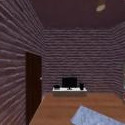
\includegraphics[width=0.9\textwidth]{04/l1_ex01.jpg}
            \caption{}
    \end{subfigure}%
    \hfill
    \begin{subfigure}[t]{0.3\textwidth}
            \centering
            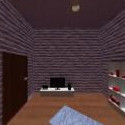
\includegraphics[width=0.9\textwidth]{04/l1_ex02.jpg}
            \caption{}
    \end{subfigure}
    \hfill
    \begin{subfigure}[t]{0.3\textwidth}
            \centering
            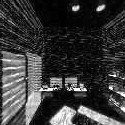
\includegraphics[width=0.9\textwidth]{04/l1_ex03.jpg}
            \caption{L1 error visualization of (a) and (b)}
    \end{subfigure}%
    \hfill
    \hfill
  \caption[Example visualization of L1 RGB error]{Example visualization of L1 RGB error. The RGB error values have been intensified so that they are more visible.} \label{fig:l1_example}
\end{figure}

As in the case of optical flow calculation, some adjustment must be made to adapt this metric for 360\degree images. Since the equirectangular projection is not equal-area, the areas towards the poles would intrinsically have higher weighting, since RGB L1 is calculated per pixel. To avoid this problem, the cube map projection is used, since it does not significantly distort the image. The average value is then calculated using the six faces of the cube, omitting the black background.

\paragraph{SSIM error on Grayscale}
The other metric to complement the RGB L1 error is a variation of the the structural similarity index (SSIM) \cite{ssim}, which measures the \emph{structural similarity} between two images. Instead of comparing the images pixel by pixel, the SSIM uses the luminance, contrast and structure of the images for comparison. It compares these locally, i.e.\ it operates on smaller areas instead of the image as a whole. As a result, it is possible that the SSIM does not register small displacements in the scene if the objects are not distorted. However, the additional comparison with the RGB L1 error should mitigate this potential problem.

The SSIM metric in general, and the implementation used in the evaluation\footnote{skimage.metrics.structural\_similarity \cite{skimage}} return a value $\in [-1, 1]$ with 1 signifying an extremely similar image and -1 signifying a very different image. In order to more easily compare it with the RGB L1 error, the SSIM value is converted to an error value $ e \in [0,1]$, with 0 signifying an identical image (0 error) and 1 signifying a very different image.

The SSIM error is calculated on the grayscale image in cubemap representation. There is no need to use an RGB image, since it does not use the color values of an image. To avoid possible problems with distortion, the cubemap representation is again used.

\subsubsection{Result Analysis}
For each scenario evaluation, the number of results is made up of the dynamic parameters, the number of synthesized viewpoints, plus the baseline results. For each image, there are two error metrics to be considered.
%The number of parameters combined with the comparison to the baseline results and the use of two different error metrics results in a large number of error values.
In order to analyze these results effectively, it is necessary to break them down by creating different visualizations that highlight different attributes of the results.At first, an overview is created, from which interesting cases are selected and examined in more detail.

\paragraph{Distribution Comparison}
The first step of the analysis is a comparison of error value distribution. In order to compare all the error values of a scenario, they are plotted using a boxplot (Figure~\ref{fig:boxplot_example}). The different parameter combinations of the scenario are plotted on the y axis (e.g. viewpoint densities a, b, c) and the error distribution (i.e. the error values of all the synthesized viewpoints) is plotted on the x axis. The box plot shows the distribution of these values: the thick black line in the colored box is the median value (approx. 0.184 in Figure~\ref{fig:boxplot_example}), the colored ranges to the left and right of the median are the \ldots \todo{short description of a boxplot using the example}. Comparing the distribution of the results of a scenario gives a first general overview of the effect of the examined parameter from which interesting cases can be chosen for closer inspection.

\paragraph{Scene Analysis}
Based on the insights gained in the distribution comparison, several interesting cases are selected for closer analysis. These cases are examined by color coding the error values and assigning the colors to the positions in the scene (e.g. Figure~\ref{fig:posmap_example}). This puts the error values in context with the scene surroundings and by using the same color mapping for all the scenario results, the effect of the scenario parameters in conjunction with the scene geometry can be judged.
%, which can help with understanding the effect of the parameters on the result accuracy.

\begin{figure}
\centering
    \hfill
    \begin{subfigure}[c]{0.45\textwidth}
            \centering
            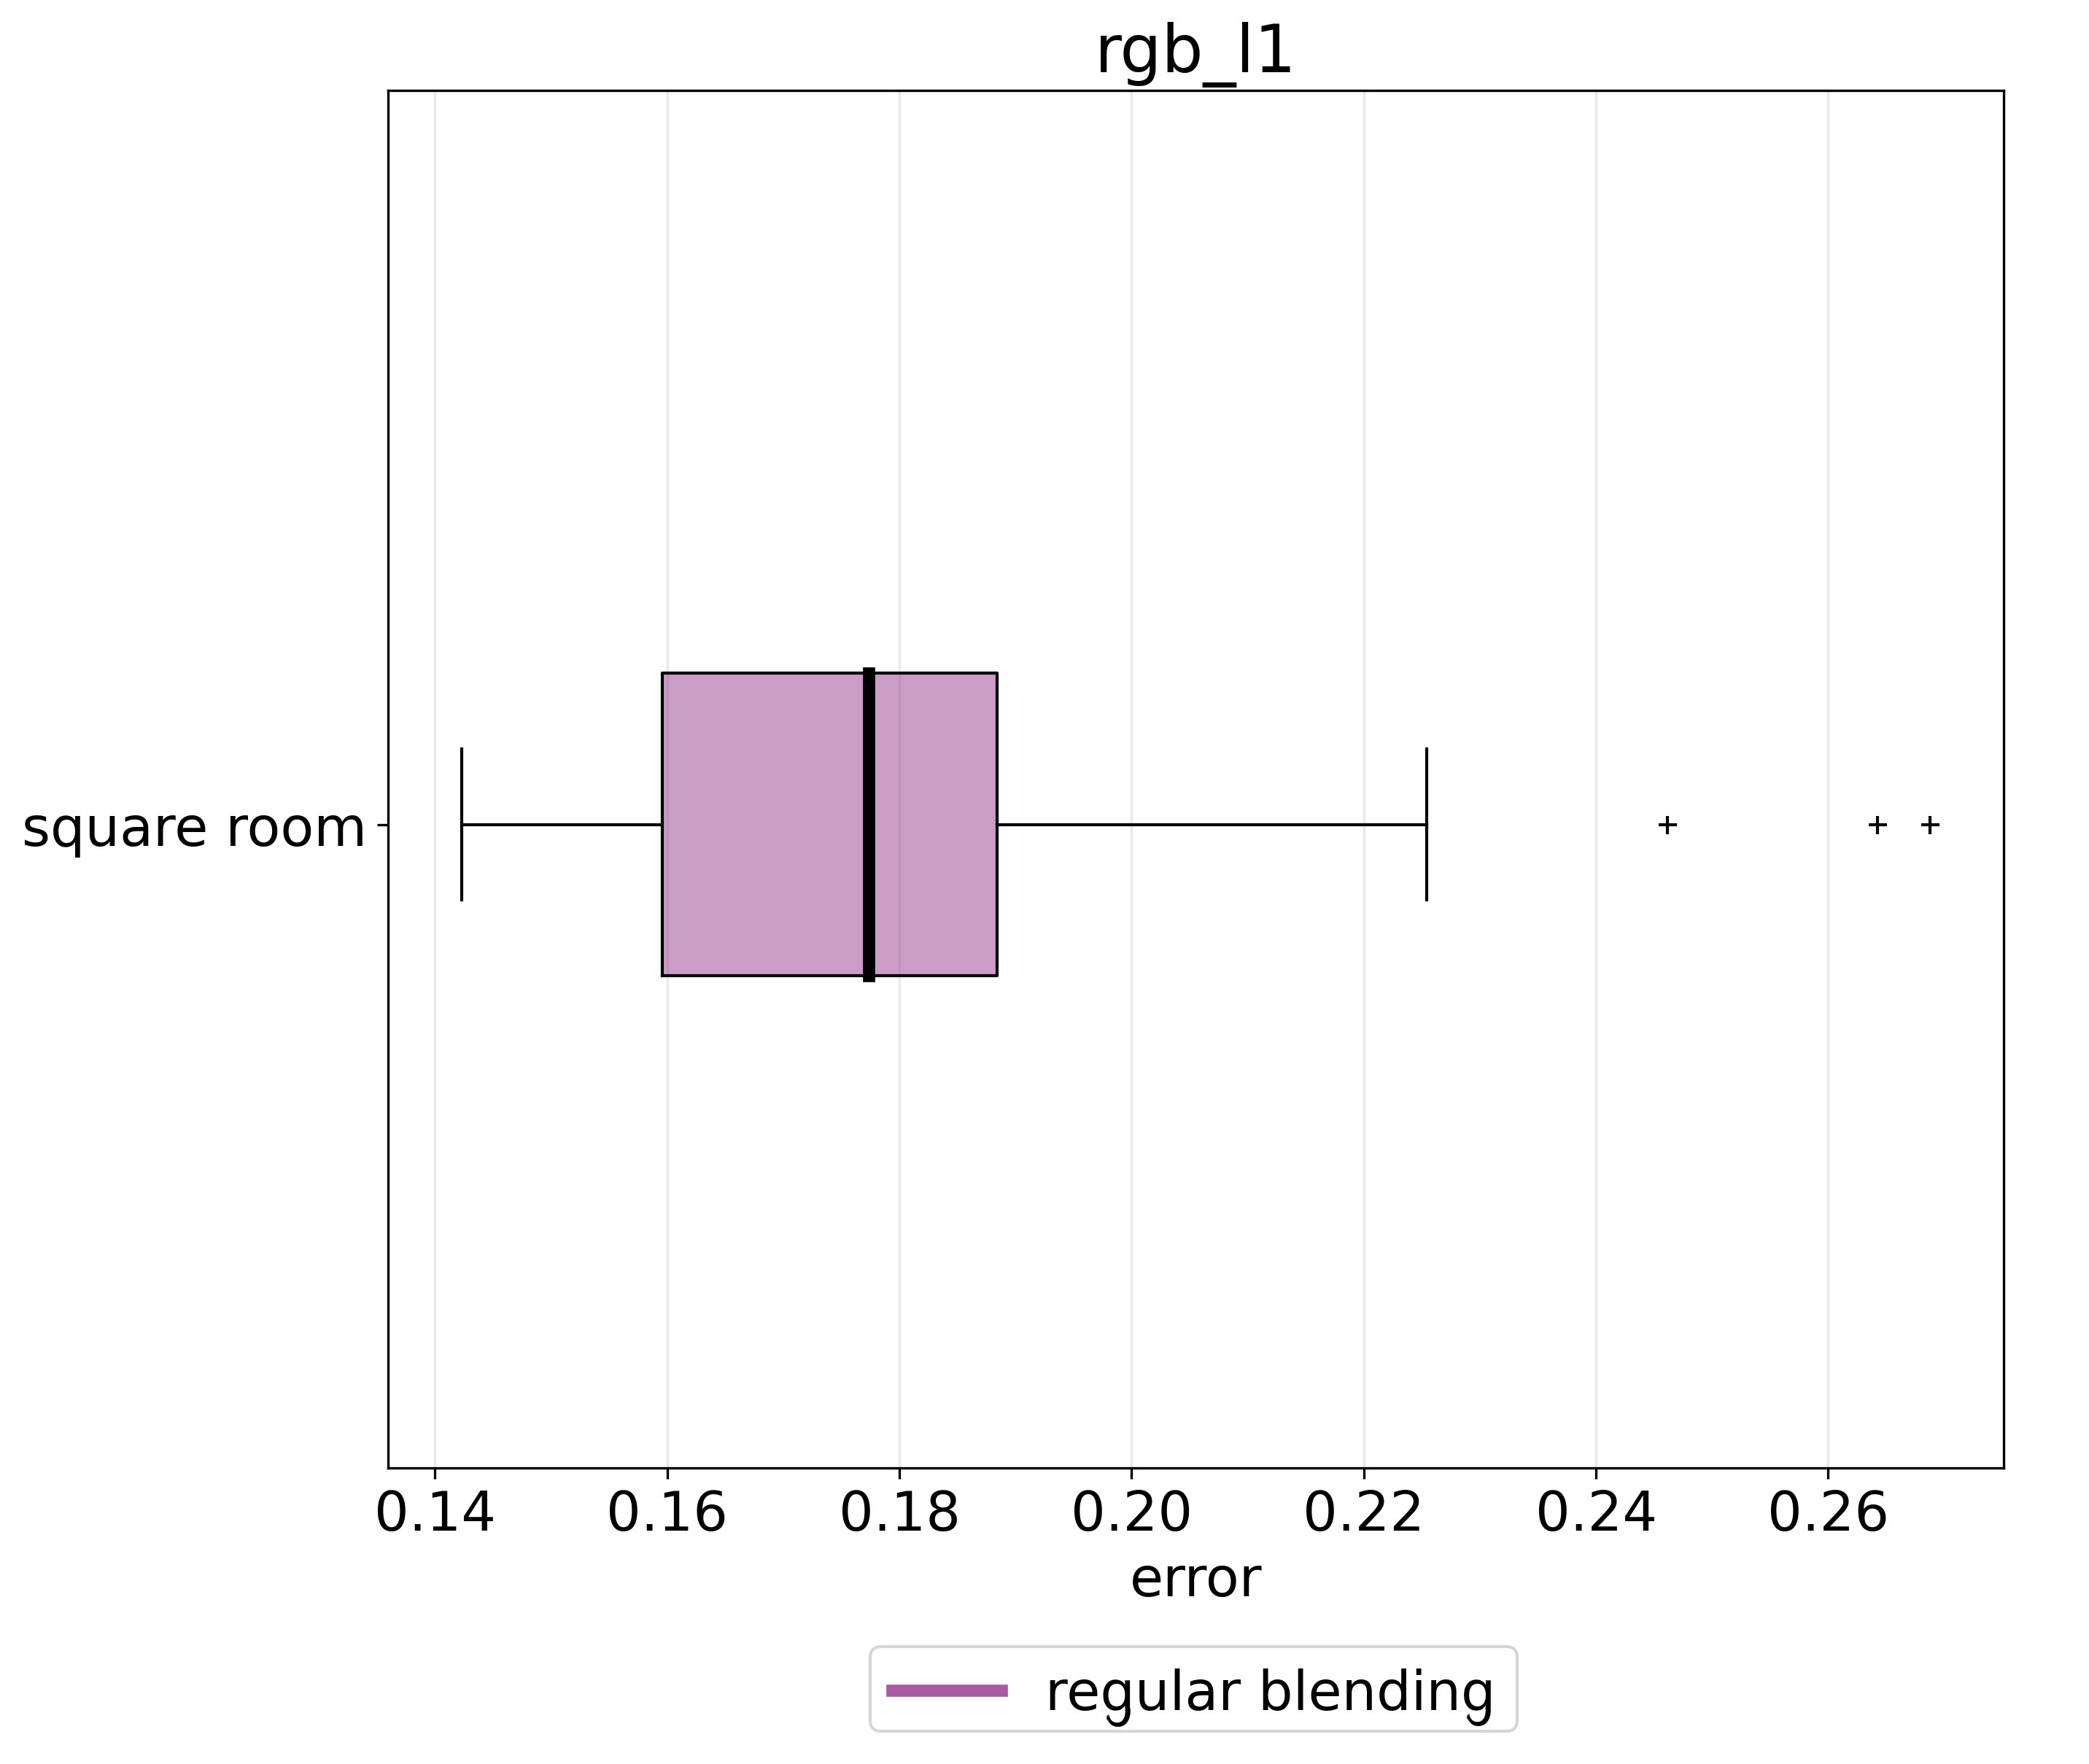
\includegraphics[width=0.9\textwidth]{04/boxplot_example.jpg}
            \caption{Boxplot example for distribution comparison} \label{fig:boxplot_example}
    \end{subfigure}%
    \hfill
    \begin{subfigure}[c]{0.4\textwidth}
            \centering
            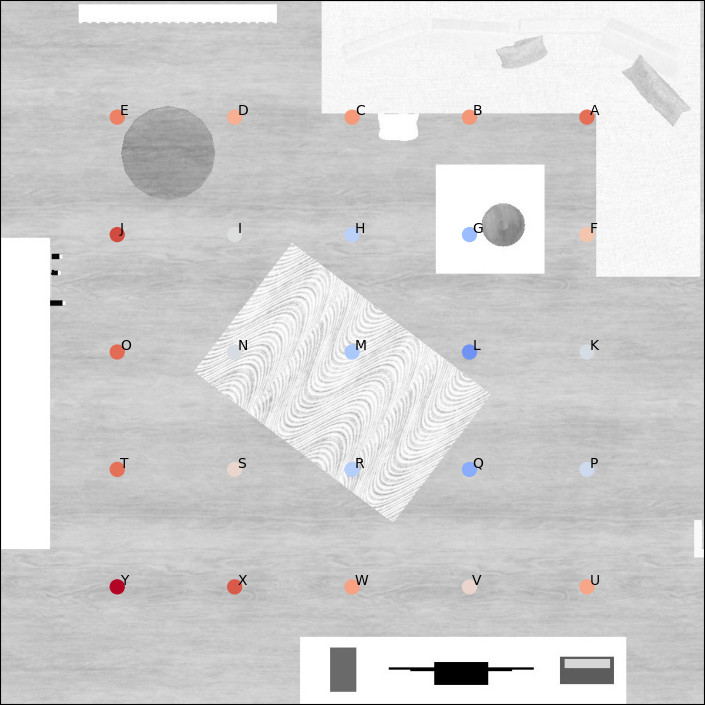
\includegraphics[width=0.9\textwidth]{04/posmap_example.jpg}
            \caption{Visualization for scene analysis: The error values are mapped to colors, with dark red representing the worst and dark blue the best value.} \label{fig:posmap_example}
    \end{subfigure}
    \hfill
  \caption{Different types of result visualization}
\end{figure}

\paragraph{Sample Inspection}
In order to further understand the effects of the parameters on specific positions, some of the synthesised viewpoints from the scene analysis are examined manually by comparing the synthesized image to the ground truth image. The manual examination may also reveal information that the error metrics are unable to extract\todo{example}.

\section{Evaluation of Limits using Virtual Scenes}
The first step of the evaluation is to test the parameters of choice in a way that explores the limits of the algorithm. In order to have full control over the scene geometry, the objects within, and the positions of the captured and synthesized viewpoints, this limit evaluation is performed on virtual scenes created with the open source 3D animation software Blender \cite{blender}.

The parameters that will be explored are:
\begin{itemize}
  \item selection of input viewpoints from the captured viewpoints
  \item flow-based blending compared to regular blending
  \item viewpoint density
  \item model-scene difference (how dissimilar is the scene geometry from the model sphere)
\end{itemize}

%Instead of testing these parameters exhaustively, specific scenarios are designed to exemplify each parameter. This reduces the testing space but also might miss some interactions between parameters. This is acceptable, since the evaluation does not aim to be comprehensive.

There is one internal parameter that is not specifically tested, but needs to be addressed, since it has a significant effect on the outcome of the flow-based blending: the optical flow algorithm. Fortunately, using virtual scenes generated with Blender can help mitigate mitigate this problem, since Blender has the capabilities to retrieve movement vectors from the geometry data, which can be used as optical flow.

\subsection{Synthesizing Ground Truth Optical Flow}
As mentioned in Section~\ref{subsec:optical_flow}, most optical flow algorithms struggle with large displacements. The flow-based blending step in the 2DoF synthesis algorithm, however, assumes perfect optical flow and there is no attempt to judge whether the optical flow calculation is feasible between two selected viewpoints. As a result, given the wrong circumstances (two viewpoints A and B that are far apart), the optical flow algorithm may fail, leading the flow-based blending to output undesirable results. The success of the optical flow algorithm is a prerequisite for the success of the 2DoF algorithm with flow-based blending.

However, the focus of this evaluation is not the accuracy of an arbitrary optical flow algorithm. In the best case, it would be possible to emulate ``perfect'' optical flow, thus decoupling the success of the optical flow from the success of the flow-based blending. While this is practically impossible for real scenes, virtual scenes theoretically contain all necessary information for retrieving ``ground truth'' optical flow. Blender, the rendering program used to create the virtual data for this evaluation, is capable of ``rendering'' motion vectors using its vector speed render pass, which calculates the movement between points from one frame to the next in pixel space. The result is a motion vector field, which corresponds to the result of a ``classic'' optical flow algorithm. This ``ground truth'' optical flow was first presented by Butler et al.\ \cite{sintel} as a benchmark for optical flow algorithms.

Figure~\ref{fig:calc_vs_synth_flow} shows the results of 1DoF interpolation with calculated flow compared to the results using optical flow synthesized by Blender. All captured viewpoints were generated in the same virtual room, with different distances between viewpoints A and B. 25 different viewpoints in in a regular grid were interpolated for this test\todo{compare viewpoint to viewpoint to see if all results are actually better}, \ldots

\begin{figure}
		\centering
		\includegraphics[width=\textwidth]{04/calc_vs_synth_flow2.png}
		\caption{Comparing 1DoF Interpolation using Calculated Flow vs Blender Flow}
		\label{fig:calc_vs_synth_flow}
\end{figure}

It is notable that the results using Blender's optical flow tend to have a smaller error value than the results using calculated optical flow, which is expected. It may seem surprising that the results are not perfect, given ``ground truth'' optical flow. However, unfortunately, the accuracy of the 1DoF interpolation is limited, even with ``ground truth'' optical flow provided by Blender. There are several possible reasons for this, mostly based on the fact that the process in Blender, like most optical flow algorithms, is designed for frame-to-frame use. Nevertheless, no definitive explanation can be made at this point, since this would require in-depth understanding of Blender's vector speed render pass, which is outside of the scope of this thesis. Based on the results shown in Figure~\ref{fig:calc_vs_synth_flow}, and experience gained from testing both variants, the Blender optical flow is used for the limit evaluation, because, even though it is not perfect, it still seems to yield better results than Scipy's implementation of Farneb\"ack's optical flow algorithm and as such decouples (to a degree) the succes of the 2DoF synthesis with flow-based blending from the success of the optical flow algorithm.

%\begin{itemize}
%   \item points that are not visible because of perspective shift will not have a correspondence
%   \item distortion due to wide fov may have an effect on the results
%   \item even blender motion vectors are for frame to frame use, so it is possible, that large jumps do not work well because the blender algo can't handle it
%\end{itemize}

\subsection{Scenarios and Results}

\subsubsection{Viewpoint Density and Choice of Viewpoints to be Synthesized}
- different densities
- want to be able to compare them to each other \ar same synthesized viewpoints with different densities \ar need controllable distances to the synthesized viewpoints
One simple way of doing this is to choose a grid of ground truth viewpoints and captured viewpoints so that the captured viewpoints are always at equal distances to the ground truth points. This is fulfilled with a grid of 5x5 ground truth viewpoints and grids of 6x6 and 12x12 captured viewpoints.

\subsubsection{Selection of Input Viewpoints}
input selection and scenes are var, all others are fixed
using only two input vps with synthesized point on the line is equal to using only 1DoF interpolation
\begin{verbatim}
Hypothesis: 2vps is better for flow-based, radius is better for regular.
flow based does not do well with image patches with different viewpoint indices
(extreme discontinuities)

Test: 
  -use the two simplest scenes with a medium number of viewpoints and synthesize using
only two vs all within the radius of 1/2*scene radius

Show: 
  - compare flow to flow and regular to regular
      --> we only want to know which is better for each blending method,
      not in comparison

Even if the hypothesis is not proven, or is not very distinct,
can still argue that >2 or >4 is computationally too costly for consideration

\end{verbatim}

\subsubsection{Viewpoint density effect on flow-based blending and regular blending}
density, blending var, others fixed
\begin{verbatim}
Hypothesis: higher density --> better results, but difference is larger for flow-based.
(optional: High density and 2vps may be better than 4)

Hypothesis II: the effect of higher density is more marked near walls and corners

Test:
  - use square room and test 2x2, 6x6, 10x10
  - compare flow with flow, reg with flow, and reg with reg -> 3 graphs

\end{verbatim}

\subsubsection{Flow-based blending vs regular depending on model-scene difference}
blending and scene var, others fixed
\begin{itemize}
  \item ``checkersphere'' in which the scene model exactly matches the scene
    \ar reprojection will yield exact results (excluding resolution)
  \item explain why it will yield correct results and why the resolution is not perfect
\end{itemize}
\begin{verbatim}
Hypothesis: the closer the scene is to the model, the better regular blending is.
the farther away, the worse it is and the better flow-based blending is

Test: compare the two with their respective better vp selection in the different scenes

\end{verbatim}


\section{Proof-of-Concept Evaluation using Real Scenes}

\section{Discussion}

\subsection{Limits}

limits of the evaluation:
\begin{itemize}
  \item interactions between the parameters are not closely examined \ar possible that some parameter affects another in an unexpected way
  \item objects are not clearly classified/measured, so no quantifiable evaluation possible
  \item positional and rotational knowledge may be calculable by sfm algos, but we don't know what kind of impact accuracy of the metadata will have, since we are hand-recording metadata meticulously
  \item pixel differences and ssim give no indication on human perception, so it is not possible to judge believability
  \item even though the results suggest it, cannot be sure that the metrics measured are significant/robust
  \item all gt points are exactly in the middle of input points (except 2x2) this has a definite effect on optical flow interpolation, especially between 2 viewpoints
  \item interactions between different parameters are not examined exhaustively, so no conclusive information
\end{itemize}

\begin{itemize}
  \item choice of gt points \ar fixed
  \item \ar offset of synth point from the line between two points (this would measure the effect of th 2DoF approximation
  \item distance from captured point (in the scenes, the gt points are always the furthest possible distance from all other points)
  \item optical flow accuracy in relation to the scene size etc
\end{itemize}
limitations also here?

Assuming radius accuracy does in fact make a slight assumption about the scene geometry. Using only the deviation angle will lead to ``spots'' where the distance is fairly large but the angle is zero. 

\subsection{Future Work}
\begin{itemize}
  \item ``guess'' an optimal radius without using viewpoint locations e.g. outside
  \item find a good weight function that balances deviation angle and distance appropriately
  \item use methods like SLAM in order to be independent of actually recording metadata by hand
  \item undistort extended cubemap e.g. by using methods like \cite{fov} which can undistort images up to 120\degree
  \item extend to 3D \ar input viewpoints could improve flow-based blending for areas towards the poles
  \item parallelization and offloading to gpu
  \item improve choice of $\delta$
  \item human perception evaluation with user study
\end{itemize}

